\subsection{OSI参照モデル}

インターネットで利用されるプロトコルは、The Internet Engineering Task Force (IETF)という標準化
団体により策定され、その標準はRequest for Comments (RFC)という名のオープンな仕様として発行されている。
例えば、我々が利用しているインターネットプロトコルである
インターネットプロトコル バージョン4は、1981年に791番目のRFCとして策定された~\cite{RFC0791}。

IETF以外の通信に関する標準化団体としては
International Telecommunication Union Telecommunication Standardization Sector (ITU-T)や、
International Organization for Standardization (ISO)が存在する。
実は、1977年から1982年かけて、ITU-TやISOがコンピュータネットワークの標準通信プロトコルとして、
Open Systems Interconnection (OSI)の策定を行っていた。
その当時は標準的な通信プロトコルは存在せず、ベンダーごとに様々なプロトコルが利用されていたため、
通信プロトコルの統一化が求められていたのである。
しかしながら、最終的にOSIは主流とはならず、IETFによって策定された
インターネットプロトコルが広く利用されるようになっていった。

\begin{figure}[tb]
    \centering
    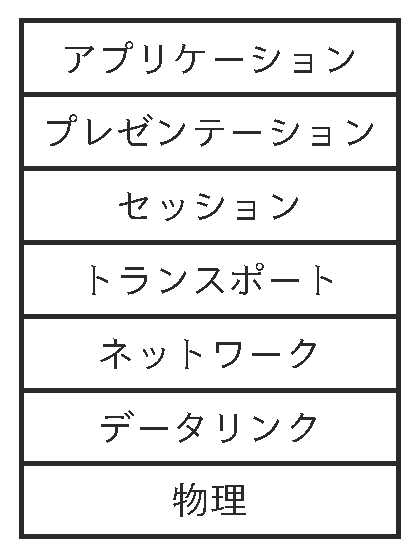
\includegraphics[width=5cm,pagebox=artbox]{figs/OSI.pdf}
    \caption{OSI参照モデル}
    \label{fig:osi}
\end{figure}

OSI自体は残らなかったが、OSI策定の際に考案されたOSI参照モデルと呼ばれる
ネットワークの抽象化手法は、今日でも広く受け入れられている。
図~\ref{fig:osi}は、OSI参照モデルによるネットワークの抽象化モデルを表している。
OSI参照モデルでは、ネットワークの機能を階層構造にもとづいて抽象化しており、
この抽象化をレイヤリングなどと呼ぶ。
OSI参照モデルでは、下から順に1層に物理層、2層にデータリンク層、
3層にネットワーク層、4層にトランスポート層、5層にセッション層、
6層にプレゼンテーション層、7層にアプリケーション層が位置する。
ちなみに、各層のことをレイヤ1、レイヤ2といったり、更に略してL1、L2などということもある。

\begin{figure}[tb]
    \centering
    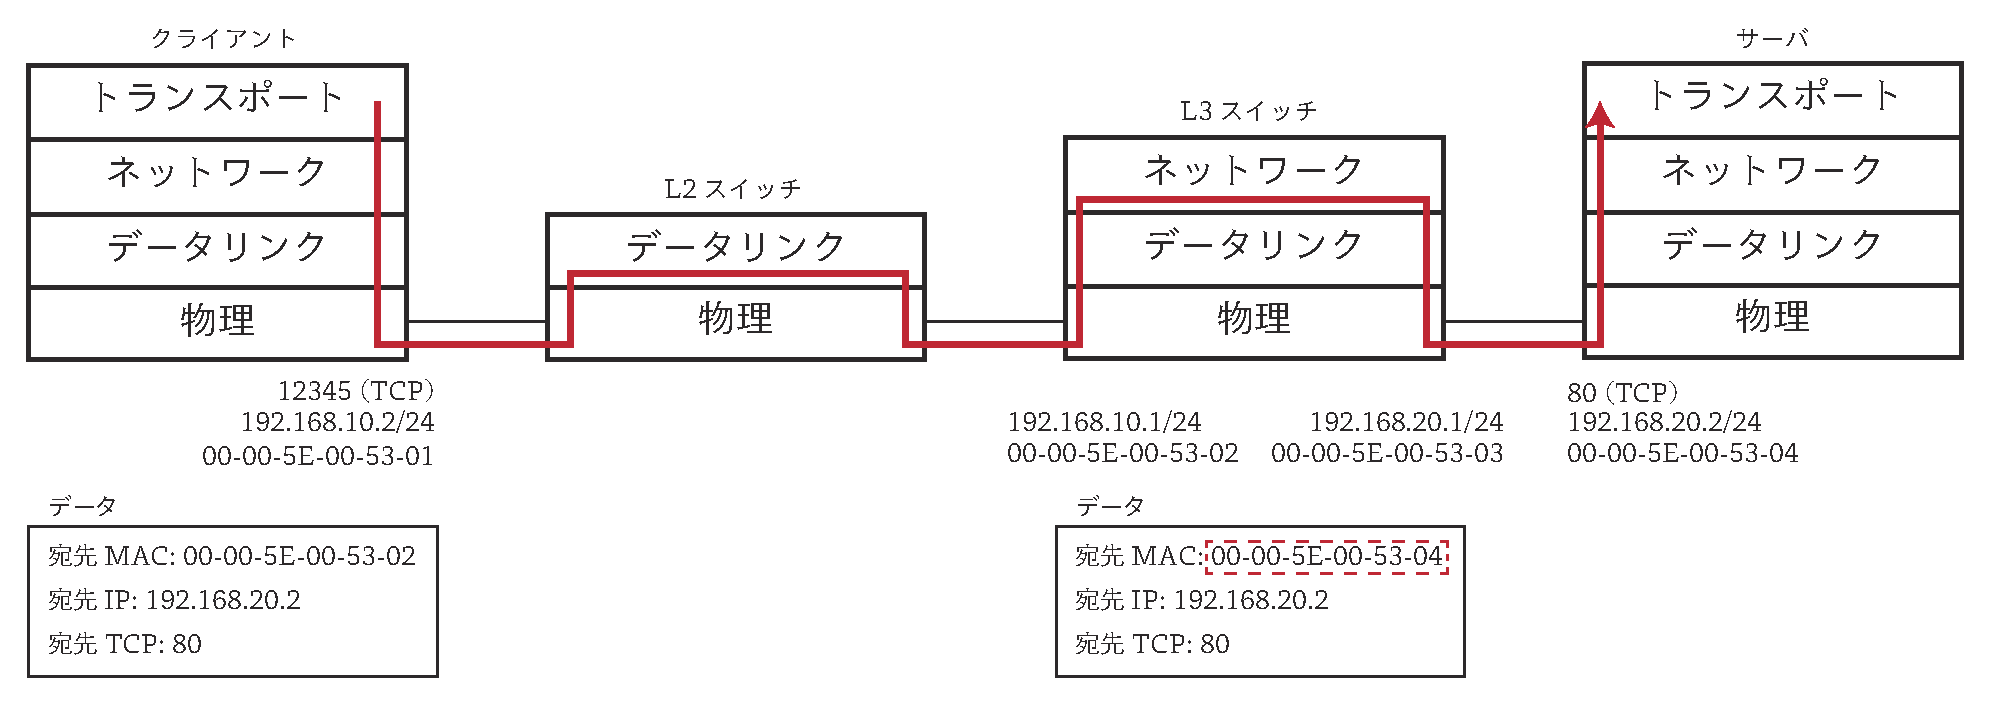
\includegraphics[width=14cm,pagebox=artbox]{figs/osi_link.pdf}
    \caption{各層でのデータ転送}
    \label{fig:osi_link}
\end{figure}

図~\ref{fig:osi_link}は各層でデータ転送が行われている様子を示している。
\footnote{
この図の意味することは現時点では理解できないかもしれないが、
この図の意味することろを説明するのが本節の目標であるため、
現段階で理解できなくても問題ない。
}
データリンク、ネットワーク、トランスポート層のプロトコルにはそれぞれアドレスがあり、
各層は、そのアドレスに基づいて転送を行う。
データリンク層プロトコルの一つであるIEEE 802では、アドレスは42ビットで表され、16進数で表現すると00-00-5E-00-53-02といった
表記になる。
図~\ref{fig:osi_link}中で宛先MACと示される値は、
IEEE 802の宛先MACアドレスを示している。
なお、MACは Media Access Controlの略である。
データリンク層は、ローカルなネットワークでの通信を行うために用いられる。
そのため、MACアドレスはそのローカルな環境では一意に識別できる必要がある。
データリンク層の詳細については~\ref{sec:datalink}節で解説する。

ネットワーク層プロトコルの一つであるIPのアドレスは、192.168.10.2/24という32ビットの数値で表され、
/24はネットワークのサブネット長を示している。
図~\ref{fig:osi_link}では、192.168.10.0/24と192.168.20.0/24
というサブネットが示されている。
IPは、全世界で通信を行うために用いられるプロトコルであり、
基本的にはIPアドレスは世界で一意に識別できるように割り当てるのが設計理念となっている
(現実的にはそうはなっていないが)。
なお、前述のアドレスはIPv4アドレスであるが、IPv6の場合は128ビットのアドレス空間を持つ。
ネットワーク層の詳細については~\ref{sec:network}節で解説する。

トランスポート層プロトコルのTCPとUDPのアドレスは16ビットで示され、一般的にポート番号と呼ばれ、
TCPやUDPはポート番号をもとにアプリケーションプロセスの識別を行う。
よく利用されるポート番号は、インターネット上で利用される識別情報の管理割当を行っている
Internet Assigned Number Authority (IANA)が定義しており~\cite{wellknown}、
一般的にこのようなポート番号をWell Knownポート番号と呼ぶ。
例えば、TCPの80番ポートはHTTPで利用され、普段我々がWebを閲覧する際は、
WebブラウザがWebサーバのTCP80番ポートへ接続する。

図~\ref{fig:osi_link}では、クライントからサーバのTCP80番ポートへむけて
通信を行っている様子を示している。
一般的に、インターネット上の通信ではデータ中に含まれる各層のアドレスをもとに、
L2またはL3スイッチが転送を行う。
L2スイッチのことをスイッチングハブといったり、
L3スイッチのことをルータということもあるが、本書ではL2スイッチ、
L3スイッチと呼ぶことにする。
この図が示すように、L2スイッチ、L3スイッチによってデータが転送されても、
データ中のIPアドレスとポート番号は変わらないが、MACアドレスはL3スイッチでの転送時に更新される。
これは、MACアドレスはローカルなネットワーク内でのみ通用するアドレスであり、
L3スイッチはローカルなネットワーク同士をつなぎ合わせる役割を持っているためである。
以降の節では、データリンク、ネットワーク、トランスポートの動きについて詳しく説明する。

\begin{itembox}[l]{\bf 重要ポイント}
    \begin{itemize}
        \item インターネット関連のプロトコルは、IETFが発行するRFCによって標準化されている
        \item コンピュータネットワークはレイヤで考えることができる
        \item Ethernetのアドレスは48ビットのMACアドレス、IPv4のアドレスは32ビットのIPv4アドレス、IPv6のアドレスは128ビットのIPv6アドレス、TCPとUDPのアドレスは16ビットのポート番号
    \end{itemize}
\end{itembox}

\subsection{おもちゃのネットワークスタック} \label{sec:stack}

\begin{figure}[tb]
    \centering
    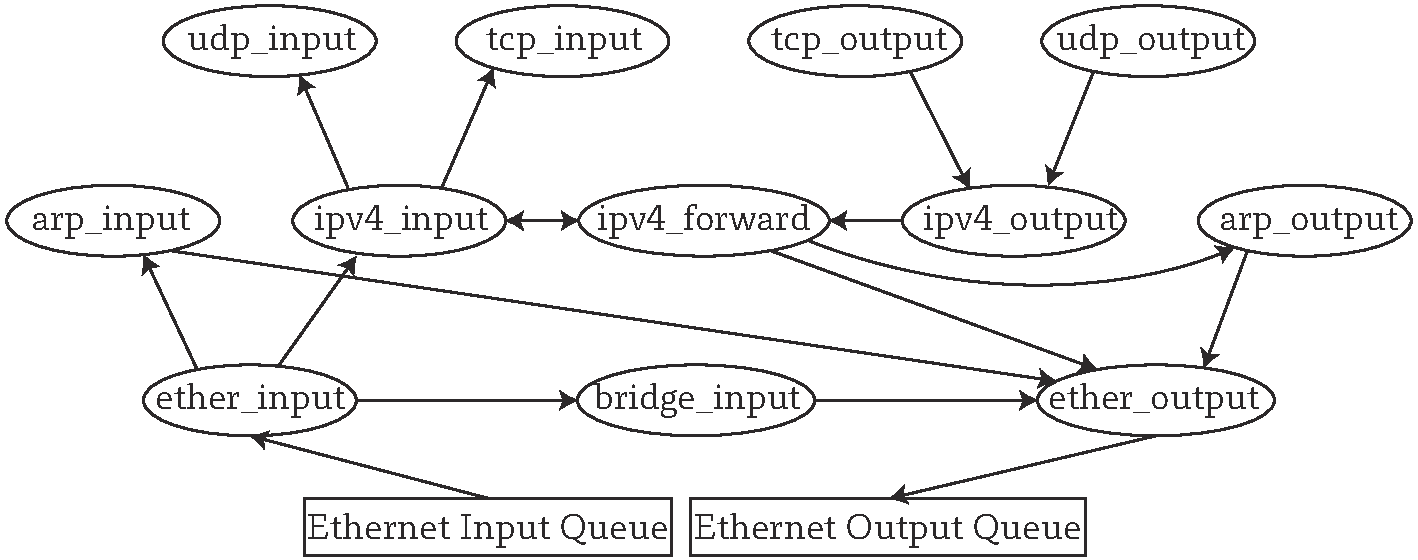
\includegraphics[width=14cm,pagebox=artbox]{figs/nwstack.pdf}
    \caption{おもちゃのネットワークスタックのデータフロー図}
    \label{fig:tcpipstack}
\end{figure}

これより本章では、おもちゃのネットワークスタックを用いて、
ネットワークスタックの設計と実装を解説する。
おもちゃと言っても、実際にIPルータやEthernetブリッジとして動作するれっきとしたネットワークスタックである。
図~\ref{fig:tcpipstack}はおもちゃのネットワークスタックのデータフロー図を示している。
この図の下部には、入力と出力用のEthernet Input/Ouptput Queueというキューがあり、
ここで物理的な入出力が行われる。
実際に、ネットワークインターフェースカードには入出力用のキューが用意されており、
デバイスドライバはこれらキューに対して読み書きすることでデータの送受信を行う。

なお、このおもちゃのネットワークは、Ethernetブリッジや、IPv4のルーティングは行うことができるが、
TCPのセッション管理などは行えないし、扱えるのは基本的にIPはユニキャストのみで、IPマルチキャスト通信はサポートしていない。
また、実際のOSではネットワークスタックの上にソケットレイヤが配置され、
ネットワークに関する操作が抽象化されているが、おもちゃのネットワークスタックではソケットレイヤは省略されている。
すなわち、あくまでも、ネットワークスタックの仕組みから理解してファイアウォールなどを運用するために必要最低限と思われる機能のみが実装されている。

\subsection{ネットワークインターフェース} \label{sec:nwif}

スタックの説明を行う前に、ネットワークインターフェース情報を表すための構造体を説明しよう。
ソースコード~\ref{src:my_ifnet.h}は、おもちゃのネットワークスタックで定義するネットワークインターフェース用のmy\_ifnet構造体となる。

\begin{lstlisting}[caption=ネットワークインターフェースを表す構造体 (my\_ifnet.h),label=src:my_ifnet.h]
// インターフェース情報を保持する構造体
struct my_ifnet {
    int idx;                       // インデックス
    uint8_t ifaddr[6];             // MACアドレス
    struct in_addr addr;           // IPv4アドレス
    struct in6_addr addr6;         // IPv6アドレス
    uint8_t plen;                  // IPv4プレフィックス長
    uint8_t plen6;                 // IPv6プレフィックス長
    char infile[128];              // 入力UNIXファイル名
    char outfile[128];             // 出力UNIXファイル名
    int sockfd;                    // 入力先UNIXドメインソケット
    struct sockaddr_un outun;      // 出力UNIXアドレス
    LIST_ENTRY(my_ifnet) pointers; // リスト
};
\end{lstlisting}

my\_ifnet構造体のメンバ変数は基本的にはコメントにあるとおりだが、もう少し詳しく説明したのが
表~\ref{tab:my_ifnet}となる。
表~\ref{tab:my_ifnet}で示すように、ネットワークインターフェースには各種アドレスが紐付けられる。
また、おもちゃのネットワークスタックでは、データの送受信にUNIXドメインソケットのデータグラム通信を行うため、
UNIXドメインソケット用のデータがいくつが用意されている。

\begin{table}[tb]
    \centering
    \caption{my\_ifnet構造体のメンバ変数} \label{tab:my_ifnet}
    \begin{tabular}{rl}
        idx & 複数インターフェースの番号を識別するためのメンバ変数 \\
        addr & インターフェースに対応付けられたIPv4アドレス \\
        addr6 & インターフェースに対応付けられたIPv6アドレス \\
        plen & IPv4プレフィックスアドレス(\ref{sec:network}節にて解説) \\
        plen6 & IPv6プレフィックスアドレス(\ref{sec:network}節にて解説) \\
        infile & データ受信を行うためのUNIXドメインソケットへのファイル名 \\
        outfile & データ送信を行うためのUNIXドメインソケットへのファイル名 \\
        sockfd & データ受信用のUNIXドメインソケットへのデスクリプタ \\
        outun & データ送信用のUNIXドメインソケットへのアドレス \\
        pointers & 複数インターフェースをリストで管理するためのポインタ。sys/queue.hを利用 \\
    \end{tabular}
\end{table}

ソースコード~\ref{tab:my_ifnet}はおもちゃのネットワークスタックの割り込みハンドラを表している。
割り込みハンドラとは、ネットワークカードにデータが到着した際に呼び出される関数のことを指す。
実際のOSでは物理的な入力が割り込みハンドラを起動するが、おもちゃのネットワークスタックでは
UNIXドメインソケットへの入力があったときにdev\_input関数を呼び出すようにしている。

\begin{lstlisting}[caption=割り込みハンドラ (my\_ifnet.c),label=src:my_ifnet.c]
/*
 * インターフェース入力割り込み関数
 * 引数:
 *   fd: UNIXドメインソケットへのファイルデスクリプタ
 */
void dev_input(int fd) {
    for (struct my_ifnet *np = LIST_FIRST(&ifs); np != NULL;
         np = LIST_NEXT(np, pointers)) {
        if (np->sockfd == fd) {
            char buf[4096];
            ssize_t size;
        again:
            size = recv(fd, buf, sizeof(buf), 0);
            if (size < 0) {
                if ((errno) == EAGAIN)
                    goto again;

                perror("recv");
                break;
            }

            ether_input(np, (struct ether_header *)buf, size);
            break;
        }
    }
}
\end{lstlisting}

ソースコード~\ref{tab:my_ifnet}では引数に入力用のUNIXドメインソケットを受け取り、
7〜8行目で対応するUNIXドメインソケットを持つmy\_ifnet構造体をリストから検索している。
入力インターフェースのmy\_ifnet構造体が見つかったら(9行目)、13行目でデータ読み込みを行っている。
14〜20行目エラー処理で、読み込みに失敗した場合はerrnoがEAGAINであれば、再度読み直し
それ以外であれば読み込み失敗として関数を抜ける。
データを読み込んだ後、22行目でether\_input関数を呼び出して実際の処理に入る。
これは図~\ref{fig:tcpipstack}で示される、Ethernet Input Queueからether\_input関数へのデータフローに相当する。

\begin{itembox}[l]{\bf 重要ポイント}
    \begin{itemize}
        \item ネットワークインターフェースカードにデータが到着した際に、OSで設定した割り込みハンドラと呼ばれる関数が呼び出される
        \item 割り込みハンドラから、実際にネットワーク処理を行うための関数が呼ばれる
    \end{itemize}
\end{itembox}

\subsection{データリンク層} \label{sec:datalink}

ソースコード~\ref{src:ethernet.h}はEthernet (IEEE 802.3) プロトコルのヘッダ構造体を示している。
我々が普段利用している無線や有線のEthernetでは、内部的にはこのようなフォーマットのヘッダがデータの先頭に付与され、
その後にIPヘッダ、TCPヘッダなどのより上位のヘッダが続き、最後にアプリケーションデータが続く。
もう少し正確に言うと、ソースコード~\ref{src:ethernet.h}で示すEthernetヘッダの前にプリアンブルなどの
ハードウェアで利用されるデータが続くが、本書ではその説明は割愛する。

\begin{lstlisting}[caption=Ethernetプロトコルヘッダ定義 (/usr/include/net/ethernet.h),label=src:ethernet.h]
#define ETHER_ADDR_LEN  6       /* Ethernet address length              */

/*
 * The length of the combined header.
 */
struct  ether_header {
        u_int8_t  ether_dhost[ETHER_ADDR_LEN];
        u_int8_t  ether_shost[ETHER_ADDR_LEN];
        u_int16_t ether_type;
};

#define ETHERTYPE_IP            0x0800  /* IP protocol */
#define ETHERTYPE_ARP           0x0806  /* Addr. resolution protocol */
#define ETHERTYPE_IPV6          0x86dd  /* IPv6 */
\end{lstlisting}

ソースコード~\ref{src:ethernet.h}で示されるように、
Ethernetヘッダの構造体は、OpenBSDでは、/usr/include/net/ethernet.h にて定義されている。
なお、以降特に断りがない限り対象とするOSはOpenBSDとし、/usr/includeのパスから始まるソースコードは、
OSが提供するソースコードであるとする。
1行目のETHER\_ADDR\_LENでは、Ethernetアドレス(MACアドレス)のバイト数を6バイトと定義している。
6行目以降がEthernetヘッダを示すether\_header構造体となる。
ether\_header構造体では、ether\_dhostとether\_shostというメンバ変数を持ち、
それぞれ宛先MACアドレスと送信元MACアドレスを示している。
ether\_typeメンバ変数は、Ethernetヘッダ以降に続くプロトコル種類を示している。

ether\_typeメンバ変数で利用できる値はIANAによって定義されている~\cite{ieee802}。
例えば、IPv4が続く場合は16進数表記で0x0800という値がether\_typeに格納される。
他には、IPv6の場合は0x08DD、仮想的なLANを構築するためのIEEE 802.1Q VLANプロトコルの場合は0x8100が格納される。
この値はether\_header構造体と同じファイルにて定義されており、
ソースコード\ref{src:ethernet.h}に12〜14行目に一部抜粋してある。
ただし、ether\_typeメンバ変数のバイトオーダはビッグエンディアンであるため、
比較や格納する際はバイトオーダを変換してから行わなければならない。

ソースコード~\ref{src:ether_input}はおもちゃのネットワークスタックのEthernetフレームを受け取り処理を行うethernet\_input関数である。
この関数では、引数に入力インターフェースを指すmy\_ifnet構造体のポインタ、入力Ethernetフレームへのポインタ、フレーム長をとり、
Ethernetヘッダ中のプロトコルタイプに応じて上位レイヤの関数に渡している。

\begin{lstlisting}[caption=ether\_input関数 (ether.c),label=src:ether_input]
// ADDRがIPv4ブロードキャストアドレスなら真、それ以外なら偽を返すマクロ
#define IS_BROADCAST(ADDR)                                                     \
    (((ADDR)[0] == 0xFF) && ((ADDR)[1] == 0xFF) && ((ADDR)[2] == 0xFF) &&      \
     ((ADDR)[3] == 0xFF) && ((ADDR)[4] == 0xFF) && ((ADDR)[5] == 0xFF))

/*
 * Ethernetフレーム入力関数
 * 引数:
 *   ifp: 入力インターフェース
 *   eh: 入力フレーム
 *   len: 入力フレーム長
 */
void ether_input(struct my_ifnet *ifp, struct ether_header *eh, int len) {
    printf("ether_input:\n");
    printf("    IF#: %d\n", ifp->idx);
    printf("    SRC MAC: %02X-%02X-%02X-%02X-%02X-%02X\n", eh->ether_shost[0],
           eh->ether_shost[1], eh->ether_shost[2], eh->ether_shost[3],
           eh->ether_shost[4], eh->ether_shost[5]);
    printf("    DST MAC: %02X-%02X-%02X-%02X-%02X-%02X\n", eh->ether_dhost[0],
           eh->ether_dhost[1], eh->ether_dhost[2], eh->ether_dhost[3],
           eh->ether_dhost[4], eh->ether_dhost[5]);
    printf("\n");

    if (IS_BROADCAST(eh->ether_dhost)) {
        // ブロードキャストアドレスの場合、ブリッジ処理へ
        if (IS_L2BRIDGE)
            bridge_input(ifp, eh, len);
    } else if (memcmp(ifp->ifaddr, eh->ether_dhost, ETHER_ADDR_LEN) != 0) {
        // 宛先MACアドレスが自インターフェース宛でないならブリッジ処理を行い終了
        if (IS_L2BRIDGE)
            bridge_input(ifp, eh, len);
        return;
    }

    switch (ntohs(eh->ether_type)) {
    case ETHERTYPE_IP: // IPv4入力
        ipv4_input((struct ip *)((uint8_t *)eh + ETHER_HDR_LEN));
        break;
    case ETHERTYPE_IPV6: // IPv6入力
        ipv6_input((struct ip6_hdr *)((uint8_t *)eh + ETHER_HDR_LEN));
        break;
    case ETHERTYPE_ARP: // ARP入力
        arp_input(ifp, (struct arphdr *)((uint8_t *)eh + ETHER_HDR_LEN));
        break;
    default:
        printf("eh->ether_type is neither IPv6 nor IPv6\n");
        return;
    }

    return;
}\end{lstlisting}

14〜22行目では入力Ethernetフレームの送信元と宛先MACアドレスを表示している。
24行目では、宛先がブロードキャストアドレスかチェックしている。
すなわち、FF-FF-FF-FF-FF-FFというMACアドレスがEthernetのブロードキャストアドレスであるため、
この値かどうかを、IS\_BROADCASTマクロで判定している。
宛先がブロードキャストアドレスの場合かつ、L2ブリッジが有効であるなら、
L2ブリッジ処理を行うbridge\_input処理を行い、自身のネットワークスタック入力処理へと進む。
28行目では、宛先が受信したネットワークインターフェースのMACアドレスと同じであるか
(すなわち自分宛てであるか)をチェックし、自分宛てで無いならば、L2ブリッジが有効の場合に
L2ブリッジ処理を行う関数へデータを渡し、ether\_input処理を終了する。
L2ブリッジが有効かどうかは、IS\_L2BRIDGEというマクロで判定する。

35行目から始まるswitch文では、上位のレイヤのプロトコルタイプを判別して、
対応するプロトコルの関数に渡している。
おもちゃのネットワークスタックでは、IPv4のみに対応しているが、
例のためにIPv6用のダミー関数も用意している。
また、IPv4で通信を行うためには、アドレス解決プロトコル(Address Resolution Protocol、ARP)~\cite{RFC0862}
というプロトコルでMACアドレスとIPv4アドレスの対応の解決を行わなければならない。
そのため、おもちゃのネットワークスタックでもARPをサポートしている。

なお、ETHERTYPE\_IP、ETHERTYPE\_IPV6、ETHERTYPE\_ARPといった定義は、
ソースコード~\ref{src:ethernet.h}で示したように、/usr/include/net/ethernet.hで定義されている。
35行目ではntohsという関数を利用するが、これは2バイト変数のバイトオーダを
ホストバイトオーダ(ホストCPUに依存)からからネットワークバイトオーダ(ビッグエンディアン)に
変換する標準Cライブラリ関数となる。

\begin{itembox}[l]{\bf 重要ポイント}
    \begin{itemize}
        \item 入力インターフェースのMACアドレスと、Ethernetヘッダ中の宛先MACアドレスを比較して、自身宛てのEthernetフレームか判別する
        \item ブロードキャストMACアドレス(FF-FF-FF-FF-FF-FF)の場合は自身宛てと判別する
        \item Ethernetヘッダ中のプロトコルタイプフィールドを判別して、IPv4、IPv6、ARPなど上位層のプロトコル種別を判別する
    \end{itemize}
\end{itembox}

\subsection{L2ブリッジ} \label{sec:l2bridge}

\begin{figure}[tb]
    \centering
    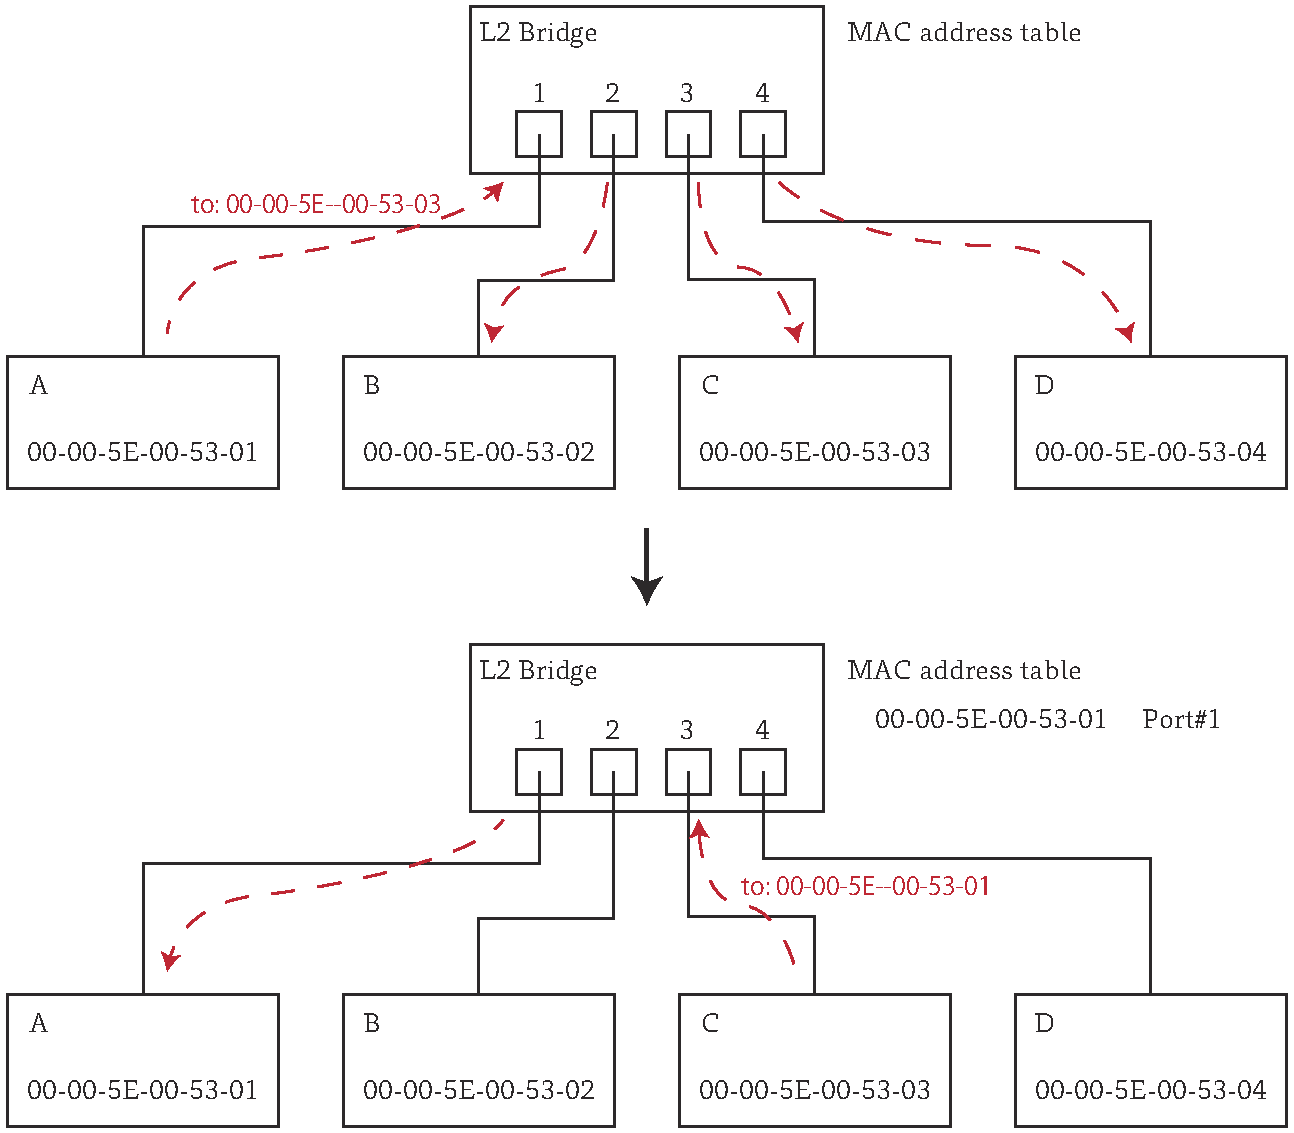
\includegraphics[width=14cm,pagebox=artbox]{figs/bridge.pdf}
    \caption{L2ブリッジの動作図}
    \label{fig:bridge}
\end{figure}

図~\ref{fig:bridge}はL2ブリッジの動作を示した図となる。
L2ブリッジにはポートと呼ばれる物理的~\footnote{仮想的な場合もある}なポートと呼ばれる接続口があり、
それぞれのポートと各ホストが接続されている。
また、一般的にL2ブリッジはMACアドレステーブルと呼ばれるテーブルを保持しており、
このMACアドレステーブルはMACアドレスとポート番号を保持している。

図~\ref{fig:bridge}では、4つのノードA〜Dが、1つのL2ブリッジに接続されており、
初期状態ではL2ブリッジのMACアドレステーブルは空の状態である。
図の上部ではホストAからホストCのMACアドレス00-00-5E-00-53-03へ向けて
Ethernetフレームが送信され、このEthernetフレームはL2ブリッジにより
全てのホストへ向けて転送されている。
これは、L2ブリッジがEthernetフレームを転送する際には、転送すべきポートを
MACアドレステーブルから参照して決定するが、
MACアドレステーブルにMACアドレスが存在しない場合は、全てのポートへ転送するためである。

L2ブリッジは、一度Ethernetフレームを転送するとEthernetフレームの送信元MACアドレスとポート番号を記憶する。
これを示したのが図~\ref{fig:bridge}の下部のMACアドレステーブルとなる。
本図の下部では、Ethernetフレームを受け取ったホストCが、
ホストAのMACアドレスである00-00-5E-00-53-01に対して何かしら応答している。
しかし、ここではL2ブリッジは全てのホストへ向けてEthernetフレームを転送するのではなく、
ホストAのみに対して転送されている。
これは、MACアドレステーブルにすでにホストAのMACアドレスとポート番号が保存されているためである。

ソースコード~\ref{src:mactable}は、おもちゃのネットワークでのMACアドレステーブルの実装を
示している。
\begin{lstlisting}[caption=MACアドレステーブルの実装,label=src:mactable]
// MACアドレスのハッシュ値を計算するマクロ
#define MACHASH(ADDR)                                                          \
    ((ADDR)[0] ^ (ADDR)[1] ^ (ADDR)[2] ^ (ADDR)[3] ^ (ADDR)[4] ^ (ADDR)[5])

// MACアドレステーブル定義
struct mac2if {
    uint8_t addr[ETHER_ADDR_LEN];
    struct my_ifnet *ifp;
};

struct mac2if mactable[256]; // MACアドレステーブルのインスタンス

/*
 * MACアドレステーブルにMACアドレスを追加する関数
 * 引数:
 *   ifp: 入力インターフェース
 *   eh: 入力フレーム
 */
static void add2mactable(struct my_ifnet *ifp, struct ether_header *eh) {
    // 送信元MACアドレスがブロードキャストアドレスならテーブルに追加しない
    if (IS_BROADCAST(eh->ether_shost))
        return;

    // 送信元MACアドレスからハッシュ値を計算
    uint8_t hash = MACHASH(eh->ether_shost);

    // テーブルに追加
    mactable[hash].ifp = ifp;
    memcpy(mactable[hash].addr, eh->ether_shost, ETHER_ADDR_LEN);
}

/*
 * MACアドレステーブルから対応するインターフェースを取得する関数
 * 返り値:
 *   対応するmy_ifnet構造体へのポインタ。
 *   ただし、テーブルにMACアドレスが存在しない場合はNULLが返る。
 * 引数:
 *   eh: 入力フレーム
 */
static struct my_ifnet *find_interface(struct ether_header *eh) {
    // 宛先MACアドレスからハッシュ値を計算
    uint8_t hash = MACHASH(eh->ether_dhost);

    // 送信元MACアドレスとMACアドレステーブルのMACアドレスとを比較
    if (memcmp(mactable[hash].addr, eh->ether_dhost, ETHER_ADDR_LEN) != 0)
        return NULL;

    return mactable[hash].ifp;
}
\end{lstlisting}
MACアドレステーブルは256個の配列から構成され、配列のインデックスはMACアドレスの値を排他的論理和で計算する。
ソースコード~\ref{src:mactable}の2行目は、MACアドレスのハッシュ値を計算する関数で、
5〜11行目はMACアドレステーブルの定義となる。
mac2if構造体をみてわかるように、MACアドレステーブルを利用するとMACアドレスからインターフェースを得ることが出来る。
19〜30行目で、MACアドレステーブルへ新規MACアドレスを追加するadd2mactable関数が定義されている。
また、40〜49行目では、MACアドレステーブルから、MACアドレスをキーとしてインターフェースを取得する
find\_interface関数を定義している。
これらは、11行目で定義した配列に値を格納、取得する単純な関数であるので動作は各自で確認してほしい。

ソースコード~\ref{src:bridge_input}は実際にブリッジ処理を行うbridge\_input関数となる。
この関数では、引数に入力インターフェースをさすmy\_ifnet構造体へのポインタ変数であるifpと、
入力Ethernetフレームをさすether\_header構造体へのポインタ変数であるehと、
フレーム長をさすlenをとる。
\begin{lstlisting}[caption=bridge\_input関数,label=src:bridge_input]
/*
 * ブリッジ処理を行う関数
 * 引数:
 *   ifp: 入力インターフェース
 *   eh: 入力フレーム
 *   len: 入力フレーム長
 */
static void bridge_input(struct my_ifnet *ifp, struct ether_header *eh,
                         int len) {
    // MACアドレステーブルを検索
    struct my_ifnet *outif = find_interface(eh);

    if (outif) {
        // MACアドレステーブルにキャッシュされていた場合、そのインターフェースへ送信
        ether_output(outif, eh, len);
    } else {
        // MACアドレステーブルにない場合、受信インターフェース以外の全てのインターフェースへ送信
        for (struct my_ifnet *np = LIST_FIRST(&ifs); np != NULL;
             np = LIST_NEXT(np, pointers)) {
            if (ifp != np)
                ether_output(np, eh, len);
        }
    }

    // MACアドレステーブルへキャッシュ
    add2mactable(ifp, eh);
}
\end{lstlisting}
この関数では、まず、11行目で、MACアドレステーブルを検索し出力先インターフェースを取得する。
その後、出力先インターフェースが取得できれば、15行目でそのインターフェースへ出力し、
見つからなければ18〜21行目で全てのインターフェースへ出力する。
そして最後に、26行目で、受信したEthernetフレームの送信元MACアドレスをMACアドレステーブルへ追加する。

本設では、内部にMACアドレステーブルを持つL2ブリッジについて説明したが、
MACアドレステーブルを持たず、全てのインターフェースへと転送するものもある。
一般的に、このようなL2ブリッジはリーピータハブとも呼ばれたり、バカハブ(馬鹿ハブ)とも呼んだりする。
スイッチングハブ、スマートスイッチ、インテリジェントスイッチなどと呼ぶときは全て、
MACアドレステーブルを内部的に持つが、バカハブ、リピータハブと呼ぶときには内部的にMACアドレステーブルは
持っていない。

\begin{itembox}[l]{\bf 重要ポイント}
    \begin{itemize}
        \item L2ブリッジ、スイッチングハブは、内部的にMACアドレステーブルを持ち、MACアドレスとインターフェースを結びつける
        \item Ethernetフレームの転送は、MACアドレステーブルの情報を用いて行われる 
        \item 転送すべきEthernetフレームの宛先MACアドレスがMACアドレステーブルにない場合は、全てのインターフェースへと転送する
        \item Ethernetフレームが入力されたタイミングでMACアドレステーブルが更新される
    \end{itemize}
\end{itembox}

\subsection{アドレス解決プロトコル (ARP)} \label{sec:arp}

\begin{figure}[tb]
    \centering
    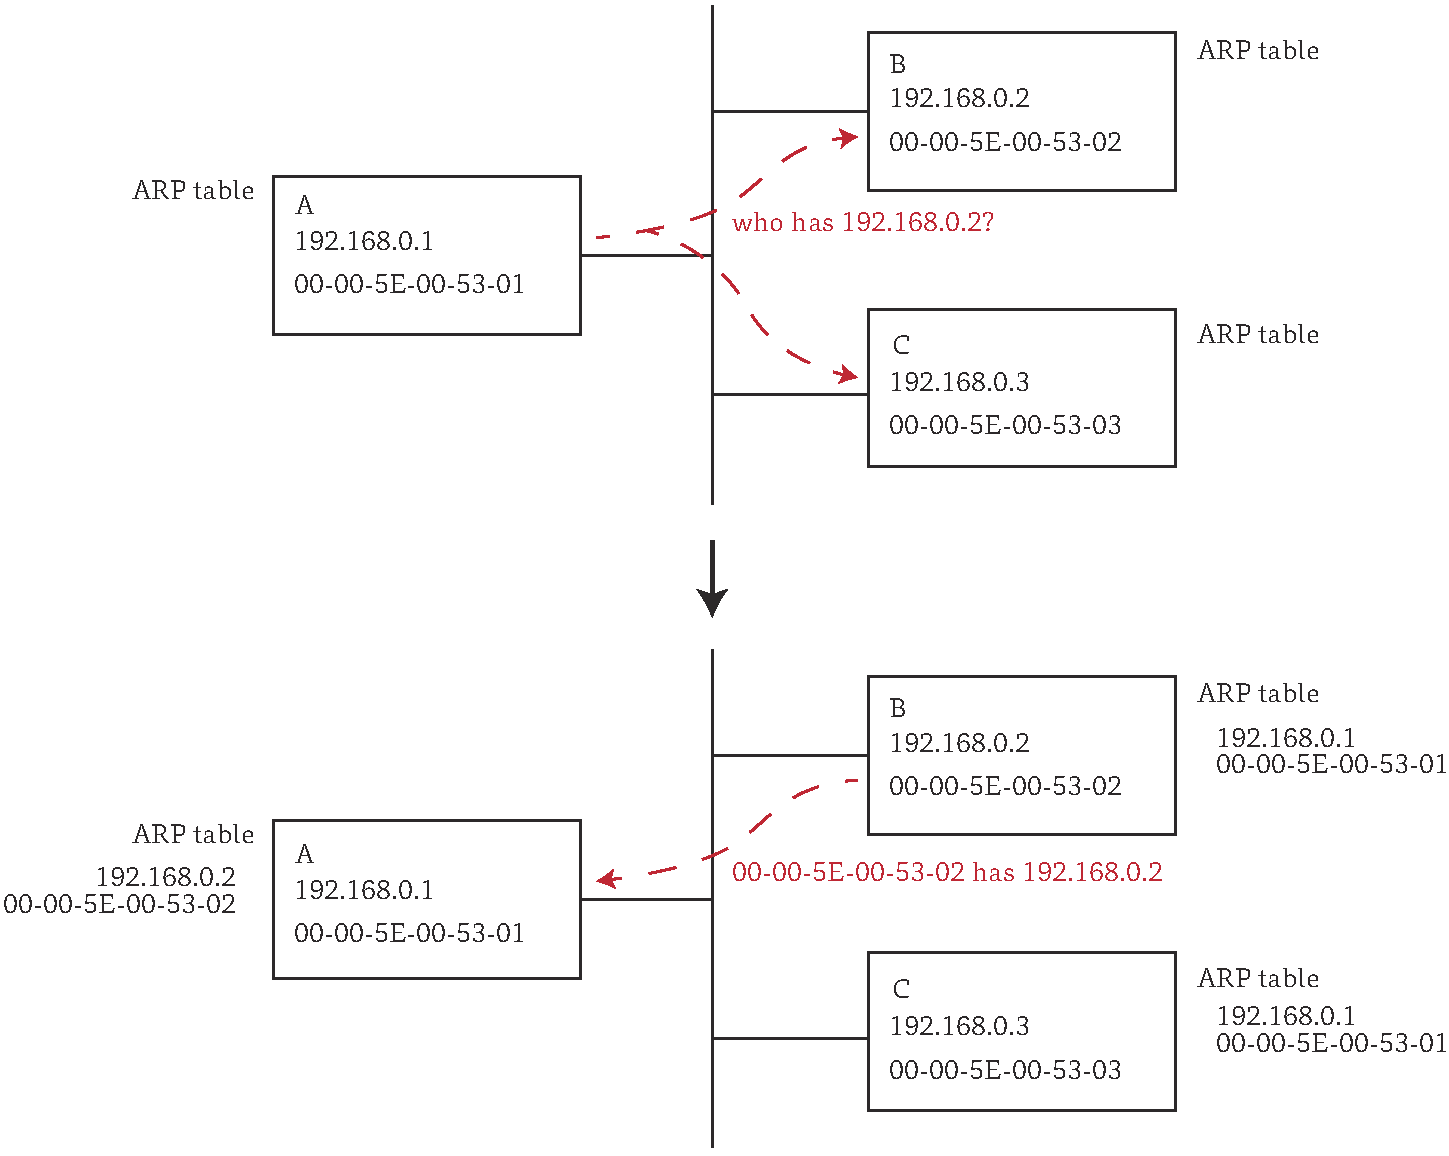
\includegraphics[width=14cm,pagebox=artbox]{figs/arp.pdf}
    \caption{ARPの動作図}
    \label{fig:arp}
\end{figure}

Ethernetでの通信はMACアドレスベースで行われる、
より上位層のIPはMACアドレスではなくIPアドレスで通信を行う。
したがって、IPパケットをEthernetフレームで転送するためには、
どのMACアドレスがどのIPアドレスに対応しているかを知らなければならない。
ARPは、IPv4アドレスからMACアドレスの対応を得るために使うプロトコルである。

図~\ref{fig:arp}はARPの動作を示した図となる。
この図では3つのホストA、B、Cがあり、AがBへと通信するためにARPでIPv4アドレスとMACアドレスの対応の
解決を行っている。
それぞれのホストはARPテーブルと呼ばれる、IPv4アドレスとMACアドレスの対応を保存しておくテーブルを持っており、
初期状態ではARPテーブルは空である。

ホストAがホストBに通信を行うために、ホストAは、まずARPリクエストと呼ばれるパケットを
Ethernetブロードキャストでリンク内の全てのノードに送信する
(ただしここで、ホストAはホストBのIPv4アドレスを知っているとする)。
これは図~\ref{fig:arp}の上部に赤の破線で示されるパケットであり、
このARPリクエストには、192.168.0.2というIPv4アドレスを持っているノードは誰かを問い合わせている。
ARPリクエストを受け取ったホストB、Cは自身のARPテーブルにホストAのIPv4アドレスと
MACアドレスを記憶しておく。
すると、図~\ref{fig:arp}の下部に示されるように、ホストB、CのARPテーブルが更新される。

ARPリクエストを受け取ったホストBは、リクエスト先のIPv4アドレスが自身のアドレスと一致するため、
ARPリプライをホストAに送信する。
ARPリプライを受け取ったホストAは、自身のARPテーブルにホストBの情報を追加して、
その後、実際にIPv4アドレスでの通信を開始する。

ARPヘッダ構造体とEthernetで用いるARP構造体は、ソースコード~\ref{src:if_arp.h}と\ref{src:if_ether.h}
に示すように、/usr/include/net/if\_arp.hと/usr/include/netinet/if\_ether.hにて定義されている。

\begin{lstlisting}[caption=ARP構造体 (/usr/include/net/if\_arp.h),label=src:if_arp.h]
/*
 * Address Resolution Protocol.
 *
 * See RFC 826 for protocol description.  ARP packets are variable
 * in size; the arphdr structure defines the fixed-length portion.
 * Protocol type values are the same as those for 10 Mb/s Ethernet.
 * It is followed by the variable-sized fields ar_sha, arp_spa,
 * arp_tha and arp_tpa in that order, according to the lengths
 * specified.  Field names used correspond to RFC 826.
 */
struct  arphdr {
        u_int16_t ar_hrd;       /* format of hardware address */
#define ARPHRD_ETHER    1       /* ethernet hardware format */
#define ARPHRD_IEEE802  6       /* IEEE 802 hardware format */
#define ARPHRD_FRELAY   15      /* frame relay hardware format */
#define ARPHRD_IEEE1394 24      /* IEEE 1394 (FireWire) hardware format */
        u_int16_t ar_pro;       /* format of protocol address */
        u_int8_t  ar_hln;       /* length of hardware address */
        u_int8_t  ar_pln;       /* length of protocol address */
        u_int16_t ar_op;        /* one of: */
#define ARPOP_REQUEST   1       /* request to resolve address */
#define ARPOP_REPLY     2       /* response to previous request */
#define ARPOP_REVREQUEST 3      /* request protocol address given hardware */
#define ARPOP_REVREPLY  4       /* response giving protocol address */
#define ARPOP_INVREQUEST 8      /* request to identify peer */
#define ARPOP_INVREPLY  9       /* response identifying peer */
/*
 * The remaining fields are variable in size,
 * according to the sizes above.
 */
#ifdef COMMENT_ONLY
        u_int8_t  ar_sha[];     /* sender hardware address */
        u_int8_t  ar_spa[];     /* sender protocol address */
        u_int8_t  ar_tha[];     /* target hardware address */
        u_int8_t  ar_tpa[];     /* target protocol address */
#endif
};
\end{lstlisting}

\begin{lstlisting}[caption=Ethernet用ARP構造体 (/usr/include/netinet/if\_ether.h),label=src:if_ether.h]
/*
 * Ethernet Address Resolution Protocol.
 *
 * See RFC 826 for protocol description.  Structure below is adapted
 * to resolving internet addresses.  Field names used correspond to
 * RFC 826.
 */
struct  ether_arp {
        struct  arphdr ea_hdr;  /* fixed-size header */
        u_char  arp_sha[ETHER_ADDR_LEN];        /* sender hardware address */
        u_char  arp_spa[4];     /* sender protocol address */
        u_char  arp_tha[ETHER_ADDR_LEN];        /* target hardware address */
        u_char  arp_tpa[4];     /* target protocol address */
}
\end{lstlisting}

\begin{table}[tb]
    \centering
    \caption{arphdr構造体のメンバ変数(全てビッグエンディアン)} \label{tab:arphdr}
    \begin{tabular}{rl}
        ar\_hrd & L2プロトコル識別子。Ethernetの場合は1 \\
        ar\_pro & L3プロトコル識別子。IPv4の場合はETHERTYPE\_IP \\
        ar\_hln & L2アドレスのバイト数。MACアドレスの場合は6バイト \\
        ar\_pln & L3アドレスのバイト数。IPv4アドレスの場合は4バイト \\
        ar\_op & ARPの種類。リクエストの場合は1で、リプライの場合は2 \\
    \end{tabular}
\end{table}

表~\ref{tab:arphdr}はarphdr構造体のメンバ変数を説明した表となる。
基本的に、ar\_op変数以外の値はEthernetとIPv4を扱うときは表で示した値で固定となる。
ただし、構造体定義からもわかるように、ARPはEthernetやIPv4に限らず様々なプロトコルで利用可能な設計となっている。
ether\_arp構造体のメンバ変数は、MACアドレスとIPv4アドレスを保存する変数であることは自明のため詳細は割愛する。

次に、実際におもちゃのネットワークスタックでARP処理を行う関数を見ていく。
ソースコード~\ref{src:arp_input}は、ARPパケットを受け取り、
リクエストやリプライなどそれぞれに対応した関数を呼び出すarp\_input関数である。
\begin{lstlisting}[caption=arp\_input関数,label=src:arp_input]
/*
 * ARPリクエスト及び応答を受け取る関数
 * 引数:
 *   ifp: 入力インターフェース
 *   arph: 入力ARP
 */
void arp_input(struct my_ifnet *ifp, struct arphdr *arph) {
    // Ethernet以外は未対応
    if (ntohs(arph->ar_hrd) != ARPHRD_ETHER || arph->ar_hln != ETHER_ADDR_LEN)
        return;

    // IP以外は未対応
    if (ntohs(arph->ar_pro) != ETHERTYPE_IP ||
        arph->ar_pln != sizeof(struct in_addr))
        return;

    switch (ntohs(arph->ar_op)) {
    case ARPOP_REQUEST:
        // ARPリクエストを受け取り応答
        arp_req_input(ifp, arph);
        return;
    case ARPOP_REPLY:
        // リプライを受け取って送信バッファ中のフレームを送信
        arp_reply_input(ifp, arph);
        return;
    default:
        // ARPリクエストとリプライ以外は未対応
        return;
    }
}
\end{lstlisting}
arp\_input関数は引数に入力インターフェースをさすmy\_ifnet構造体へのポインタ変数であるifpと、
入力ARPパケットをさすarphdr構造体へのポインタ変数であるarphをとる。
9、10行目でL2プロトコルとL2プロトコルアドレスの長さをチェックし、Ethernetかつ6バイト意外であるなら、
未対応として処理を終了する。
13〜15行目ではL3プロトコルがIPv4であるかをチェックし、そうでないなら処理を終了する。
17行目でARPプロトコルの種類を判別し、ARPリクエストであれば20行目でarp\_req\_input関数を呼び出し、
ARPリプライであればarp\_reply\_input関数を呼び出す。
ただし、おもちゃのネットワークスタックではARPリクエストとリプライ以外は未対応であるため、
これら以外のARPパケットが来た場合は何もせずに処理を終了する。

ソースコード~\ref{src:arp_req}はARPリクエストを送信するためのarp\_req関数である。
図~\ref{fig:arp}上部のホストAは、このarp\_req関数を用いてARPリクエストを送信する。
\begin{lstlisting}[caption=arp\_req関数,label=src:arp_req]
/*
 * ARPリクエストを送信
 * 引数:
 *   ifp: 送信を行うインターフェース
 *   addr: 問い合わせを行うIPアドレスへのポインタ
 */
void arp_req(struct my_ifnet *ifp, struct in_addr *addr) {
    uint8_t buf[ETHER_HDR_LEN + sizeof(struct ether_arp)];
    struct ether_header *eh = (struct ether_header *)buf;
    struct ether_arp *req = (struct ether_arp *)(buf + ETHER_HDR_LEN);

    // Ethenerヘッダ設定
    memcpy(eh->ether_shost, ifp->ifaddr, ETHER_ADDR_LEN); // 送信元MACは自分
    memset(eh->ether_dhost, 0xff, ETHER_ADDR_LEN); // 宛先MACはブロードキャスト
    eh->ether_type = htons(ETHERTYPE_ARP);

    // ARPヘッダ設定
    req->ea_hdr.ar_hrd = ntohs(ARPHRD_ETHER); // ハードウェアタイプ (Ethernet)
    req->ea_hdr.ar_pro = ntohs(ETHERTYPE_IP); // プロトコルタイプ (IP)
    req->ea_hdr.ar_hln = ETHER_ADDR_LEN; // 6バイト。MACアドレスサイズ
    req->ea_hdr.ar_pln = sizeof(struct in_addr); // 4バイト。IPv4アドレスサイズ
    req->ea_hdr.ar_op = ntohs(ARPOP_REQUEST); // ARPリクエスト

    // ARPリクエスト設定
    memcpy(req->arp_sha, ifp->ifaddr, ETHER_ADDR_LEN); // 送信元MACは自分
    memcpy(req->arp_spa, &ifp->addr, sizeof(req->arp_spa)); // 送信元IPは自分
    memset(req->arp_tha, 0xff, ETHER_ADDR_LEN); // 宛先MACはブロードキャスト
    memcpy(req->arp_tpa, addr, sizeof(*addr)); // 問い合わせIP

    ether_output(ifp, eh, ETHER_HDR_LEN + sizeof(struct ether_arp));
}
\end{lstlisting}
arp\_req関数は出力先インターフェースをさすmy\_ifnet構造体へのポインタ変数であるifpと、
問い合わせIPv4アドレスをさすin\_addr構造体へのポインタ変数であるaddrを引数にとる。
8行目のでは送信ARPパケット用のバッファを作成しており、
9、10行目で、EthernetヘッダとARPのためのデータを格納する先のアドレスを計算している。
13、14行目ではEthernetヘッダ情報を設定しており、送信元アドレスは出力先インターフェースの
MACアドレスとしている。
その一方、宛先アドレスは、ネットワーク全体に届くようブロードキャストアドレス(FF-FF-FF-FF-FF-FF)を設定している。
また、プロトコルタイプは今回はARPであるため、ETHERTYPE\_ARPを設定している。
18〜22行目ではARPヘッダの設定をしており、これは前述したとおりである。
25〜28行目ではARPリクエストパケットにIPv4アドレスとMACアドレスを設定している。
送信元のMACとIPv4アドレスは出力先インターフェースのアドレスであり、
ターゲットのIPv4アドレスは問い合わせIPv4アドレスである。
ただし、問い合わせMACアドレスは不明なので、ここではブロードキャストに設定している。
ARPパケットに値を設定した後、最後の30行目でethernet\_output関数を呼び出し、ARPパケットを送信する。

ソースコード~\ref{src:arp_req_input}はARPリクエストを受け取りARPリプライを返信する
arp\_req\_input関数となる。
\begin{lstlisting}[caption=arp\_req\_input関数,label=src:arp_req_input]
/*
 * ARPリクエストを受け取り、ARPリプライを返す関数
 * 引数:
 *   ifp: 受信したインターフェース
 *   arph: ARPリクエストへのポインタ
 */
static void arp_req_input(struct my_ifnet *ifp, struct arphdr *arph) {
    struct ether_arp *req = (struct ether_arp *)arph;
    uint8_t buf[ETHER_HDR_LEN + sizeof(struct ether_arp)];
    struct ether_header *eh = (struct ether_header *)buf;
    struct ether_arp *reply = (struct ether_arp *)(buf + ETHER_HDR_LEN);

    char addr[16];
    inet_ntop(PF_INET, req->arp_tpa, addr, sizeof(addr));
    printf("ARP: who has %s?\n", addr);

    // ARPテーブルに追加
    add2arptable((struct in_addr *)req->arp_spa, req->arp_sha);

    // 問い合わせIPv4アドレスが自身のIPv4アドレスかチェック
    struct in_addr *tpa = (struct in_addr *)req->arp_tpa;
    if (tpa->s_addr != ifp->addr.s_addr)
        return;

    // Ethenerヘッダ設定
    memcpy(eh->ether_shost, ifp->ifaddr, ETHER_ADDR_LEN); // 送信元MACは自分
    memcpy(eh->ether_dhost, req->arp_sha, ETHER_ADDR_LEN); // 宛先MAC
    eh->ether_type = htons(ETHERTYPE_ARP);

    // ARPヘッダ設定
    reply->ea_hdr.ar_hrd = ntohs(ARPHRD_ETHER); // ハードウェアタイプ (Ethernet)
    reply->ea_hdr.ar_pro = ntohs(ETHERTYPE_IP); // プロトコルタイプ (IP)
    reply->ea_hdr.ar_hln = ETHER_ADDR_LEN; // 6バイト。MACアドレスサイズ
    reply->ea_hdr.ar_pln = sizeof(struct in_addr); // 4バイト。IPv4アドレスサイズ
    reply->ea_hdr.ar_op = ntohs(ARPOP_REPLY); // ARPリプライ

    // ARPリプライ設定
    memcpy(reply->arp_sha, ifp->ifaddr, ETHER_ADDR_LEN); // 送信元MACは自分
    memcpy(reply->arp_spa, &ifp->addr, sizeof(reply->arp_spa)); // 送信元IPは自分
    memcpy(reply->arp_tha, req->arp_sha, ETHER_ADDR_LEN);         // 宛先MAC
    memcpy(reply->arp_tpa, req->arp_spa, sizeof(reply->arp_tpa)); // 質問先IP

    ether_output(ifp, eh, ETHER_HDR_LEN + sizeof(struct ether_arp));
}
\end{lstlisting}
arp\_req\_input関数は引数に、入力インターフェースをさすmy\_ifnet構造体へのポインタ変数であるifpと、
ARPリクエストへのポインタarphをとる。
8行目では、arphポインタをether\_arp構造体へのポインタにキャストしている。
9〜11行目では、ARPリプライ用のバッファを確保し、そこからEthernetヘッダとARPリプライ構造体へのアドレスを計算している。
13〜15行目はARPリクエストの内容を表示しているのみである。
18行目はARPリクエストの情報を元にARPテーブルにデータを追加している。
これは図~\ref{fig:arp}上部でホストBとCがARPリクエストを受け取り、
下部でホストBとCが自身のARPテーブルに情報を追加している動作に相当する。
21〜23行目では、ARPリクエストの問い合わせIPv4アドレスが受信したインターフェースのIPv4アドレスかをチェックし、
自身宛でないなら処理を終了する。
26〜28行目ではEthernetヘッダの設定、31〜35行目ではARPヘッダの設定、38〜41行目ではARPリプライの設定を
行っており、最後に43行目でether\_output関数を呼び出てARPリプライを送信する。

ソースコード~\ref{src:arp_reply_input}はARPリプライを受け取り、
送信バッファで待機中のフレームを送信する関数となる。
この送信バッファは、はじめにIPv4パケットを送信する場合、ARPテーブルに対応するIPv4パケットがないため必要となる。
対応するARPエントリがない場合、一旦送信バッファに退避してからARPリクエストを送信して、
アドレス解決を行った後に退避しておいたIPv4パケットを実際に送信する。
\begin{lstlisting}[caption=arp\_reply\_input関数,label=src:arp_reply_input]
/*
 * ARPリプライを受け取り、送信バッファ中のフレームを送信する関数
 * 引数:
 *   ifp: 入力インターフェース
 *   arph:
 */
static void arp_reply_input(struct my_ifnet *ifp, struct arphdr *arph) {
    struct ether_arp *rep = (struct ether_arp *)arph;

    char addr[16];
    inet_ntop(PF_INET, rep->arp_spa, addr, sizeof(addr));
    printf("ARP: %02X-%02X-%02X-%02X-%02X-%02X has %s\n", rep->arp_sha[0],
           rep->arp_sha[1], rep->arp_sha[2], rep->arp_sha[3], rep->arp_sha[4],
           rep->arp_sha[5], addr);

    // ARPテーブルに追加
    add2arptable((struct in_addr *)rep->arp_spa, rep->arp_sha);

    // 送信バッファ中のフレームを送信
    struct sendbuf *np;
    for (np = sbuf.lh_first; np != NULL;) {
        if (np->eh->ether_type == htons(ETHERTYPE_IP)) {
            // ARPテーブルに宛先IPv4アドレスがあるか検索
            struct ip2mac *mac = find_mac(&np->nextip);
            if (mac == NULL) {
                np = np->pointers.le_next;
                continue;
            }

            // 宛先MACアドレスを設定
            memcpy(np->eh->ether_dhost, mac->macaddr, ETHER_ADDR_LEN);

            // インターフェースへ出力
            ether_output(ifp, np->eh, np->ethlen);

            // バッファを解放
            free(np->eh);
            struct sendbuf *tmp = np->pointers.le_next;
            LIST_REMOVE(np, pointers);
            free(np);
            np = tmp;
        }
    }
}
\end{lstlisting}
引数はこれまでと同じく、入力インターフェースをさすmy\_ifnet構造体へのポインタ変数であるifpと、
ARPリプライへのポインタarphである。
10〜14行目は受け取ったARPリプライを標準出力へ出力している。
17行目は受け取ったARPリプライの情報をARPテーブルに追加している。
21行目以降が送信バッファ中にあるIPv4パケットを送信する処理となる。
21行目で送信バッファを走査してIPv4パケットを取り出し、24行目で取り出したIPv4パケットの
宛先IPv4アドレスが解決されているかを検索し、
検索が失敗した場合は次のパケットへ処理を移す(25〜27行目)。
31〜34行目で、宛先MACアドレスを設定しEthernetフレームを送信している。
37行目以降は、送信済みのバッファを解放する処理となる。

\begin{itembox}[l]{\bf 重要ポイント}
    \begin{itemize}
        \item ARPを利用してIPv4アドレスとMACアドレスの解決が行われる
        \item OS内部にはIPv4アドレスとMACアドレスの対応を記録したARPテーブルが存在する
        \item ARPテーブルはARPパケットを受信したタイミングで更新される
    \end{itemize}
\end{itembox}

\subsection{IPv4} \label{sec:network}

本節ではネットワーク層のプロトコルとしてIPv4を中心に議論を行う。
IPv4以外のネットワーク層のプロトコルとしては、IPv6があるが、
IPv6については~\ref{sec:ipv6}節で簡単に説明する。
ネットワーク層のプロトコルはIPv4とIPv6以外にも、IPXなどのプロトコルがあったが現在ではほとんど使われていない。

IPv4の役目を一言で言うならば、世界中のコンピュータを一意に識別して
相互接続性を実現することである。
IPv4の識別子としては32ビットのIPv4アドレスが用いられ、
相互接続性はルーティングと呼ばれるパケット転送のメカニズムを用いて実現される。
したがって、全てのIPv4ノードは、IPv4アドレスとIPv4のルーティングテーブルを持つことになる。

\begin{figure}[tb]
    \centering
    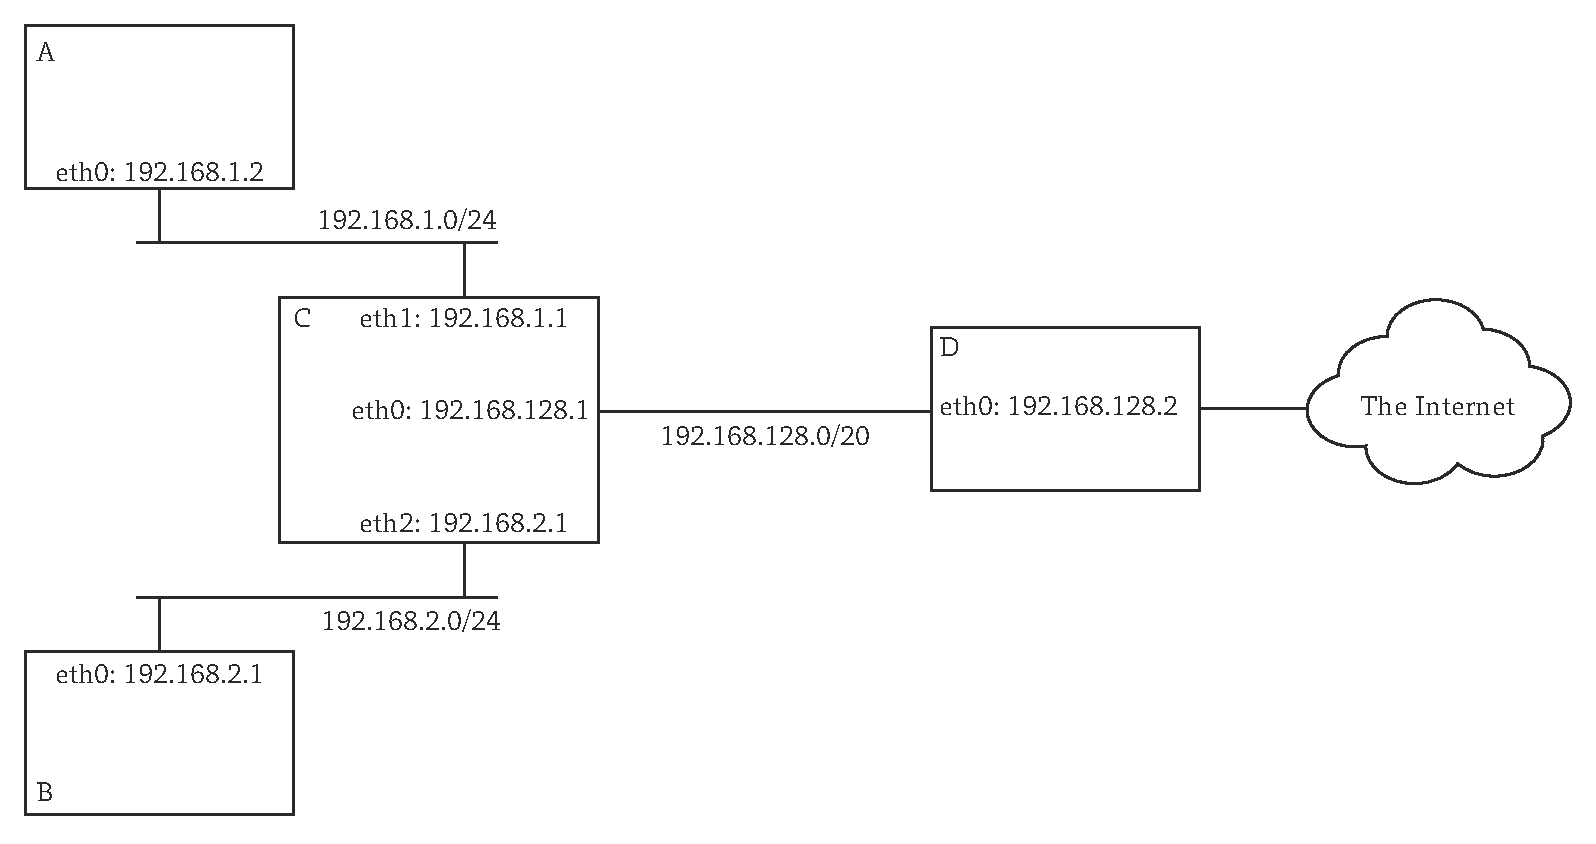
\includegraphics[width=15cm,pagebox=artbox]{figs/routing.pdf}
    \caption{IPv4のルーティング}
    \label{fig:routing}
\end{figure}

\begin{lstlisting}[caption=IPv4ヘッダ定義 (/usr/include/netinet/ip.h),label=src:ip.h]
/*
 * Structure of an internet header, naked of options.
 */
struct ip {
#if _BYTE_ORDER == _LITTLE_ENDIAN
        u_int     ip_hl:4,              /* header length */
                  ip_v:4;               /* version */
#endif
#if _BYTE_ORDER == _BIG_ENDIAN
        u_int     ip_v:4,               /* version */
                  ip_hl:4;              /* header length */
#endif
        u_int8_t  ip_tos;               /* type of service */
        u_int16_t ip_len;               /* total length */
        u_int16_t ip_id;                /* identification */
        u_int16_t ip_off;               /* fragment offset field */
#define IP_RF 0x8000                    /* reserved fragment flag */
#define IP_DF 0x4000                    /* dont fragment flag */
#define IP_MF 0x2000                    /* more fragments flag */
#define IP_OFFMASK 0x1fff               /* mask for fragmenting bits */
        u_int8_t  ip_ttl;               /* time to live */
        u_int8_t  ip_p;                 /* protocol */
        u_int16_t ip_sum;               /* checksum */
        struct    in_addr ip_src, ip_dst; /* source and dest address */
};
\end{lstlisting}

\subsection{IPv6} \label{sec:ipv6}

\begin{lstlisting}[caption=IPv6アドレス構造体 (/usr/include/netinet6/in6.h),label=src:in6.h]
/*
 * IPv6 address
 */
struct in6_addr {
        union {
                u_int8_t   __u6_addr8[16];
                u_int16_t  __u6_addr16[8];
                u_int32_t  __u6_addr32[4];
        } __u6_addr;                    /* 128-bit IP6 address */
};
\end{lstlisting}

\begin{lstlisting}[caption=IPv6ヘッダ定義 (/usr/include/netinet/ip6.h),label=src:ip6.h]
/*
 * Definition for internet protocol version 6.
 * RFC 2460
 */

struct ip6_hdr {
        union {
                struct ip6_hdrctl {
                        u_int32_t ip6_un1_flow; /* 20 bits of flow-ID */
                        u_int16_t ip6_un1_plen; /* payload length */
                        u_int8_t  ip6_un1_nxt;  /* next header */
                        u_int8_t  ip6_un1_hlim; /* hop limit */
                } ip6_un1;
                u_int8_t ip6_un2_vfc;   /* 4 bits version, top 4 bits class */
        } ip6_ctlun;
        struct in6_addr ip6_src;        /* source address */
        struct in6_addr ip6_dst;        /* destination address */
} __packed;
\end{lstlisting}

\subsection{トランスポート層} \label{sec:transport}

\begin{lstlisting}[caption=TCPヘッダ定義 (/usr/include/netinet/tcp.h),label=src:tcp.h]
typedef u_int32_t tcp_seq;

/*
 * TCP header.
 * Per RFC 793, September, 1981.
 */
struct tcphdr {
        u_int16_t th_sport;             /* source port */
        u_int16_t th_dport;             /* destination port */
        tcp_seq   th_seq;               /* sequence number */
        tcp_seq   th_ack;               /* acknowledgement number */
#if _BYTE_ORDER == _LITTLE_ENDIAN
        u_int32_t th_x2:4,              /* (unused) */
                  th_off:4;             /* data offset */
#endif
#if _BYTE_ORDER == _BIG_ENDIAN
        u_int32_t th_off:4,             /* data offset */
                  th_x2:4;              /* (unused) */
#endif
        u_int8_t  th_flags;
#define TH_FIN    0x01
#define TH_SYN    0x02
#define TH_RST    0x04
#define TH_PUSH   0x08
#define TH_ACK    0x10
#define TH_URG    0x20
#define TH_ECE    0x40
#define TH_CWR    0x80
        u_int16_t th_win;                       /* window */
        u_int16_t th_sum;                       /* checksum */
        u_int16_t th_urp;                       /* urgent pointer */
};
\end{lstlisting}

\begin{lstlisting}[caption=UDPヘッダ定義 (/usr/include/netinet/udp.h),label=src:udp.h]
/*
 * Udp protocol header.
 * Per RFC 768, September, 1981.
 */
struct udphdr {
        u_int16_t uh_sport;             /* source port */
        u_int16_t uh_dport;             /* destination port */
        u_int16_t uh_ulen;              /* udp length */
        u_int16_t uh_sum;               /* udp checksum */
};
\end{lstlisting}

\subsection{トランスポートより上の層}